
\frame{\titlepage}
\begin{frame}
  \frametitle{Innhold}
  \tableofcontents
\end{frame}

\section{Bakgrunnskunnskap}
\subsection{Felt}
\begin{frame}
  \frametitle{Felt}
  \begin{columns}
    \column{0.5\textwidth}
    \begin{itemize}
    \item \href{https://en.wikipedia.org/wiki/Field_(computer_science)}{Felt} er informasjonsbitene som er knyttet til bestemte materialer.
    \item \alert{Forfatter}, \alert{tittel}, \alert{utgivelsesår} er eksempler på felt.
    \end{itemize}

    \column{0.5\textwidth}
    \centering
    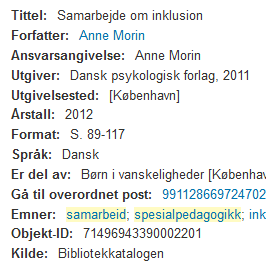
\includegraphics[width=0.8\textwidth]{../media/felt-i-oria.png}
  \end{columns}
\end{frame}

\subsection{Kontrollerte emneord}
\begin{frame}
  \frametitle{Kontrollerte emneord}
  \begin{columns}
    \column{0.5\textwidth}
    \centering
    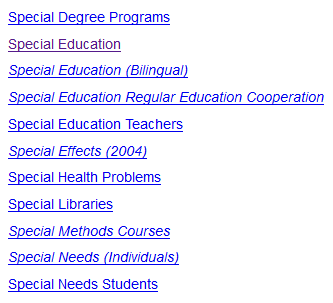
\includegraphics[width=0.8\textwidth]{../media/kontrollerte-emneord.png}

    \column{0.5\textwidth}
    \begin{itemize}
    \item \href{https://snl.no/emneord}{Kontrollerte emneord} er bestemte navneformer på bestemte emner.
    \item Kontroll på emneord tar høyde for synonymer og alternative stavelser.
    \item Siden emneordene er kontrollerte får man treff på \textit{konseptet}, ikke bare tekstbiten.
    \item Tidkrevende arbeid. Ikke alle baser tilbyr dette.
    \end{itemize}
  \end{columns}
\end{frame}

\subsection{Logiske operatorer}
\begin{frame}
  \frametitle{Logiske operatorer}
  \begin{columns}
    \column{0.5\textwidth}
    \centering
    \includegraphics<1>[width=0.5\textwidth]{../media/boolean-identity.png}
    \includegraphics<2>[width=0.5\textwidth]{../media/boolean-and.png}
    \includegraphics<3>[width=0.5\textwidth]{../media/boolean-or.png}

    \column{0.5\textwidth}
    \begin{itemize}
      \item Logiske operatorer er det samme som dagligdagse ord som \alert{og}, \alert{eller} og \alert{ikke}.
      \item Logiske operatorer brukes i søk.
      \item \textquote{Søk på dokumenter med emne \textbf{spesialpedagogikk} \alert{og} emne \textbf{barnehage*}.}
    \end{itemize}
  \end{columns}
\end{frame}

\section{Søk med nøkkelord og fulltekstsøk}
\begin{frame}
  \frametitle{Søk med nøkkelord og fulltekstsøk}
  \begin{itemize}
  \item Søk med nøkkelord og fulltekstsøk blir gjort i \alert{flere felt} (tittel, forfatter, emne) og av og til i \alert{innholdet} til artikkelen.
  \item Aktuelle søketjenester er \href{http://bibsys-almaprimo.hosted.exlibrisgroup.com/primo_library/libweb/action/search.do?vid=DMMH}{Oria}, \href{https://scholar.google.com}{Google Scholar} og \href{http://apps.webofknowledge.com}{Web of Science}.
  \end{itemize}
\end{frame}

\begin{frame}
  \frametitle{Når burde man velge nøkkelord og fulltekstsøk?}
  Nøkkelord- og fulltekstsøk er gunstige når man ønsker å inkludere mest mulig materiale blant søkeresultatene.
\end{frame}

\subsection{Nøkkelordsøk i Oria}
\begin{frame}
  \frametitle{Nøkkelordsøk i Oria}
  \begin{columns}
    \column{0.5\textwidth}
    \centering
    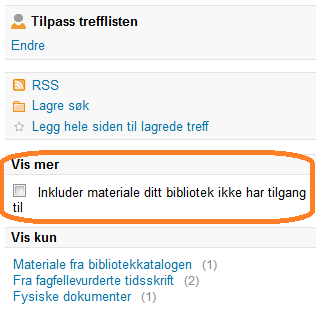
\includegraphics[width=0.8\textwidth]{../media/inkluder-materiale.png}

    \column{0.5\textwidth}
    \begin{itemize}
    \item Nøkkelordsøk i Oria passer til søk etter artikler registrert hos norske fagbibliotek, og gir ofte gode treff på skandinaviske forskningsartikler.
    \end{itemize}
  \end{columns}
\end{frame}

\subsection{Nøkkelordsøk i Google Scholar}
\begin{frame}
  \frametitle{Nøkkelordsøk i Google Scholar}
  \begin{itemize}
  \item Med Google Scholar kan du søke på tittel, forfatter, år, utgiver, tekstinnhold, osv.
  \item Søker i norske og internasjonale kilder, i alle sjangre.
  \end{itemize}
\end{frame}

\begin{frame}
  \begin{itemize}
  \item Nøkkelordsøk er standardsøket i Google Scholar.
  \item Begynn å taste nøkkelord adskilt med mellomrom for å få forslag til søk.
  \end{itemize}

  \centering
  
\includegraphics[width=0.8\textwidth]{../media/google-scholar.png}
\end{frame}

\section{Søk med kontrollerte emneord}
\begin{frame}
  \frametitle{Søk med kontrollerte emneord}
  \begin{itemize}
  \item \alert{Feltet} for emne bruker i flere litteraturdatabaser \alert{kontrollerte emneord}, og man kan utnytte dette til å finne litteratur om et bestemt emne.
  \item Hvis basen tilbyr dette får man ofte treff på de fleste relevante artikler.
  \end{itemize}
\end{frame}
\subsection{Kontrollerte emneord i ERIC}
\begin{frame}
  \frametitle{Kontrollerte emneord i ERIC}
  \begin{quote}
    The ERIC Thesaurus is a list of terms representing research topics in the field of education. Descriptors from the ERIC Thesaurus are \alert{assigned to every document} in the ERIC digital library to describe its subject content.
  \end{quote}
\end{frame}
\begin{frame}
  \centering
  
\includegraphics[width=1\textwidth]{../media/eric-descriptor.png}
\end{frame}
\begin{frame}
  \centering
  
\includegraphics[width=1\textwidth]{../media/eric-descriptor-2.png}
\end{frame}

\section{Navigering i siteringsnettverk}
\begin{frame}
  \frametitle{Navigering i siteringsnettverk}
  \begin{itemize}
    \item Navigering i siteringsnettverk kan avsløre relaterte artikler, uten at de bruker de samme nøkkelordene.
    \item Man kan finne siterte artikler, men også artikler \textit{som har sitert} den aktuelle artikkelen.
    \item Aktuelle søketjenester er \href{https://scholar.google.com}{Google Scholar} og \href{http://apps.webofknowledge.com}{Web of Science}.
  \end{itemize}
\end{frame}

\subsection{Siteringsnettverket Web of Science}
\begin{frame}
  \frametitle{Siteringsnettverket Web of Science}
  \begin{itemize}
    \item Tar for seg naturfagene, samfunnsvitenskapene og humaniora.
    \item Navigering i siterte artikler og andre dokumenter som siterer en gitt artikkel.
  \end{itemize}
\end{frame}

\begin{frame}
  \centering
  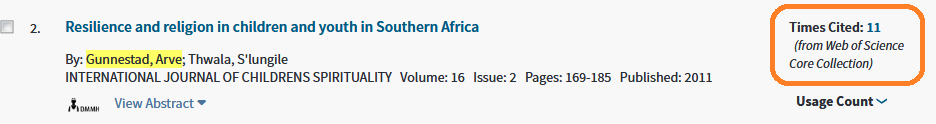
\includegraphics[width=0.8\textwidth]{../media/web-of-science-citations-2.png}
\end{frame}
